\chapter{PINEM 的能谱与相位}
\label{chap:pinem-intro}
\label{chap:pinem-core}

当一束窄能宽电子穿过被激光照明的纳米结构时，出射能谱往往在原有峰的两侧出现等间隔的增益和损失边带。间隔由光子能量 $\hbar\omega$ 决定，峰的权重却取决于电子经过结构的位置、光场相位和作用时间。这就是光子诱导近场电子显微学（PINEM）要解释的基本现象。边带不是彼此无关的吸收、发射事件：在固定轨迹和弱反冲极限中，它们是同一个周期相位因子的 Fourier 分量。我们从这一可检验的近似出发计算能谱和谱矩，再在后续章节追溯它的相对论来源及电磁边界条件。


设电子入射中心能量为 $E_0$，单色光角频率为 $\omega$。实验中把末态的能量改变记为
\begin{equation}
E_n-E_0=n\hbar\omega,\qquad n\in\ZZ.
\label{eq:intro-energy-ladder}
\end{equation}
这里 $n$ 是\emph{电子净增益阶数}：$n>0$ 表示电子获得能量，$n<0$ 表示电子损失能量。它是离散散射通道标签，并不是已经测得的光子数。若激光频率提高，峰间距增大；若电子的初始能散或仪器宽度超过 $\hbar\omega$，这些峰就会开始重叠。谱线是否可分辨与相互作用是否真的量子相干，是两个不同问题。

在经典给定场、窄能宽、弱反冲并且电子轨迹可以近似固定的条件下，离开作用区的电子振幅可写成
\begin{equation}
 c_n=J_n(2|\beta|)\ee^{\ii n\arg(-\beta)},\qquad
 P_n=|c_n|^2=J_n^2(2|\beta|).
 \label{eq:intro-pinem-spectrum}
\end{equation}
其中 $J_n$ 是第一类贝塞尔函数，$\beta$ 是无量纲复耦合。幅度 $|\beta|$ 决定有多少阶变得显著；相位 $\arg\beta$ 影响不同边带的\emph{相对相位}，但单独的能谱人口 $P_n$ 无法读出这个相位。所有边带来自一个幺正相位因子的傅里叶展开，所以必须一起满足 $\sum_nP_n=1$。即使 $|\beta|$ 增大，某一个固定阶的概率也未必单调增加；这个贝塞尔振荡特征比单纯的谱展宽更能辨认相干 PINEM。

\begin{figure}[!htbp]
\centering
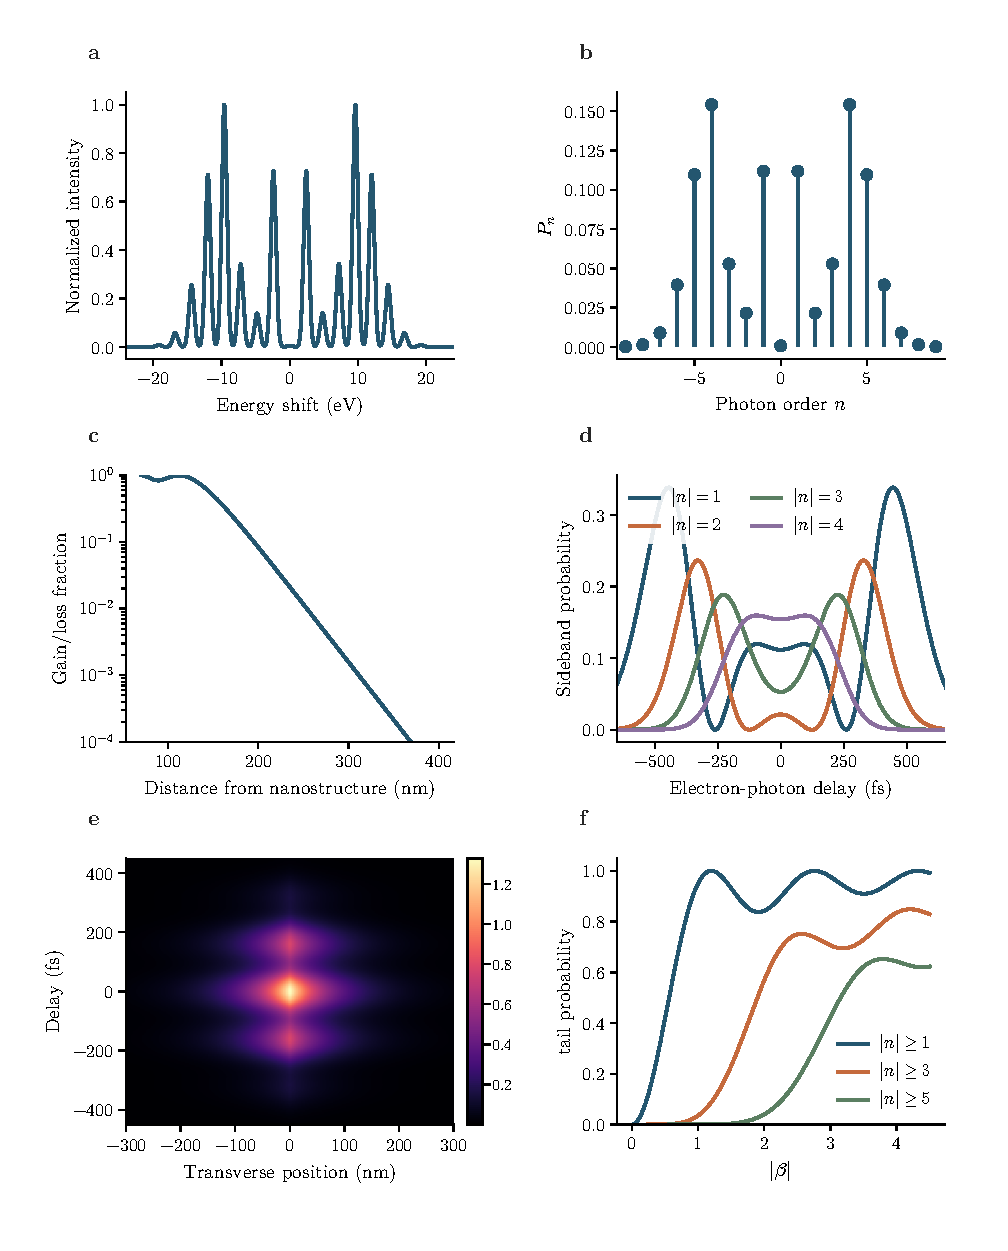
\includegraphics[width=0.97\linewidth,height=0.70\textheight,keepaspectratio]{barwick2009_foundation.pdf}
\caption{\textbf{PINEM 最初的可观测现象。} (a) 电子能谱中等间隔的增益与损失边带；(b) 同一耦合参数生成的各阶贝塞尔人口；(c) 电子远离近场结构后边带迅速减弱；(d) 改变电子与光脉冲的相对延迟得到时间门控；(e) 空间与时间共同变化的规定代理信号；(f) 提高耦合后不同高阶边带集合占据的总概率。六个面板是教学模型的前向计算，并非同一实验的原始数据。}
\label{fig:intro-pinem-observation}
\end{figure}

各面板均由同一概率模型生成。所有边带使用 $P_n=J_n^2(2|\beta|)$，相位与绝对耦合强度的定义见\cref{eq:intro-trajectory-coupling}。面板 (a) 的能量谱由单位面积高斯核对离散 $P_n$ 卷积得到，取光子能量 $2.4\,\mathrm{eV}$、$|\beta|=2.8$、$\sigma_E=0.38\,\mathrm{eV}$、$-10\le n\le10$，绘图后按最大峰高归一。(b) 绘制同一参数下的截断归一 $P_n$。(c) 使用距结构 $b\in[70,400]\,\mathrm{nm}$、$|\beta(b)|=2.8\ee^{-(b-70\,\mathrm{nm})/(50\,\mathrm{nm})}$，显示 $1-P_0$，对数轴绘图下限为 $10^{-5}$。(d) 使用延迟 $\Delta t\in[-700,700]\,\mathrm{fs}$、有效耦合 $2.8\ee^{-\Delta t^2/[4(180^2+110^2)\,\mathrm{fs}^2]}$，计算 $|n|=1,2,3,4$ 各阶概率；该有效门控不是完整电子到达时间分布的非相干平均。(e) 使用规定的无量纲代理信号 $Z(x,t)=\ee^{-|x|/(75\,\mathrm{nm})}\ee^{-[t/(230\,\mathrm{fs})]^2}[1+0.35\cos(2\pi t/(180\,\mathrm{fs}))]$，不是 Maxwell 边值求解。(f) 在 $|\beta|\in[0,4.5]$ 的 180 点扫描上，以 $|n|\le18$ 截断，分别计算 $\sum_{|n|\ge1,3,5}P_n$。


图中可以直接读出三个相互联系的实验判断。电子必须靠近受到光激发的结构，表明作用局域在近场；只有电子与光脉冲时间重叠时，边带才会明显出现；而高阶边带随着相互作用增强逐次变得可见，说明描述不能停留在最低阶微扰。这里先用\cref{eq:intro-pinem-spectrum} 读图，后面再证明它为什么是贝塞尔函数，而不是把该函数当作经验拟合式。


能量间隔只取决于 $\omega$，但各阶强度还取决于电子在哪里经过结构。电子沿 $z$ 轴以中心速度 $v$ 前进，横向撞击位置用 $\vb R$ 表示。令光场的实电场采用
\begin{equation}
\vb E(\vb r,t)=\operatorname{Re}\!\left[\vb E_\omega(\vb r)\ee^{-\ii\omega t}\right]
\label{eq:intro-field-phasor}
\end{equation}
的复相量约定，则电子在一阶轨迹近似中的无量纲耦合定义为
\begin{equation}
\beta(\vb R)=\frac{e}{2\hbar\omega}
\int_{-\infty}^{+\infty}\!\dd z\,
E_{\omega,z}(\vb R,z)\ee^{-\ii\omega z/v}.
\label{eq:intro-trajectory-coupling}
\end{equation}
这里 $e>0$ 是元电荷的大小，电子带电量为 $-e$；$E_{\omega,z}$ 是完整复相量的纵向分量，因而分母保留 $2$。若另一文献把正频电场的一半直接定义成 $E_\omega^{(+)}$，其系数会写成 $e/(\hbar\omega)$，物理结果并不相差两倍。

积分中的 $\ee^{-\ii\omega z/v}$ 是关键：电子从近场的一个位置走到另一个位置，光学振荡同时推进。不同位置对散射的贡献是\emph{复振幅相加}，不能简单把局域 $|E_z|$ 积分。如果近场沿 $z$ 近似含有 $\ee^{\ii k_z z}$，长度为 $L$ 的均匀作用区便给出
\begin{equation}
\beta\propto L\,\operatorname{sinc}\!\left(\frac{[k_z-\omega/v]L}{2}\right)
\ee^{\ii[k_z-\omega/v]L/2}.
\label{eq:intro-phase-matching}
\end{equation}
因此场中需要有接近 $k_z=\omega/v$ 的纵向傅里叶分量，这才是近场为何比普通横向自由空间光束更容易驱动同向高速电子的原因。作用区拉长会增强完全匹配时的相干积累，同时使失配容差变窄。

\begin{figure}[!htbp]
\centering
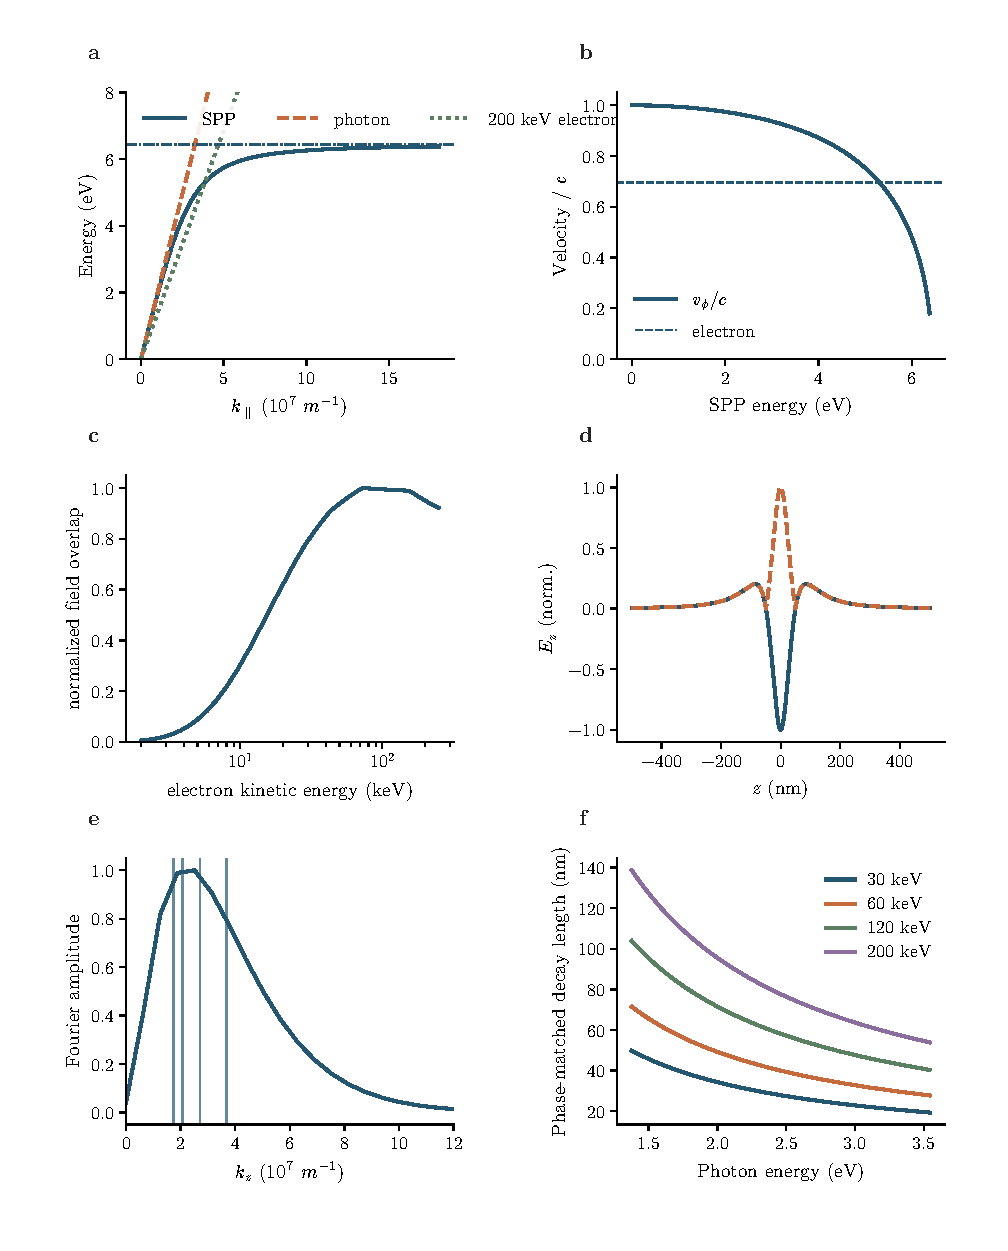
\includegraphics[width=0.97\linewidth,height=0.70\textheight,keepaspectratio]{park2010_dispersion_fourier.pdf}
\caption{\textbf{电子运动与近场傅里叶分量的配合。} (a) 光学与电子运动的色散关系；(b) 光学模式相速度与电子速度的比较；(c) 电子能量变化时所采样的纵向傅里叶幅值；(d) 用于说明匹配的偶极型纵向代理场；(e) 场的有限窗傅里叶谱及不同电子速度对应的采样位置；(f) 光学波长与电子能量共同决定的近场约束尺度。图中的色散与偶极场属于不同的理想化教学模型，不能理解为同一组 Maxwell 边界条件的自洽解。}
\label{fig:intro-phase-matching-visual}
\end{figure}

光学模式采用无耗散 Drude 介质 $\varepsilon(\omega)=1-\omega_p^2/\omega^2$ 和平面表面模式色散 $k_{\mathrm{spp}}=(\omega/c)\sqrt{\varepsilon/(1+\varepsilon)}$，取 $\hbar\omega_p=9.1\,\mathrm{eV}$。(a,b) 比较此色散及电子能量 $200\,\mathrm{keV}$ 对应的速度；(c) 扫电子动能 $K=2$--$250\,\mathrm{keV}$，在光学波长 $519\,\mathrm{nm}$ 处读取 $|\widetilde E_z(\omega/v(K))|$，按峰值归一；(d,e) 使用撞击参数 $b=70\,\mathrm{nm}$ 的规定偶极型代理场 $E_z(z)\propto [3z^2/(b^2+z^2)-1](b^2+z^2)^{-3/2}$，在 $z\in[-500,500]\,\mathrm{nm}$ 的 1000 点网格上计算离散 Fourier 变换，并叠加电子能量 $30,60,120,200\,\mathrm{keV}$ 的 $k_z=\omega/v$。(f) 在波长 $350$--$900\,\mathrm{nm}$、上述电子动能上计算模式约束长度的教学模型。所有归一与有限计算窗均属于数值设定，材料损耗尚未引入。


这时我们已经能将实验数据分成两层：谱峰位置由 $\hbar\omega$ 确定，谱峰权重由沿轨迹积累的 $\beta$ 决定。真正需要测量的并不是抽象的电场峰值，而是场在电子路径上的一个有相位的空间傅里叶分量。材料极化率、结构共振、粒子大小等因素都先通过改变这条纵向场分布，再影响能谱。由此也能看出，图中的代理场可以帮助认识趋势，却不能替代特定纳米颗粒的严格电磁场求解。


理想谱是离散概率 $P_n$，实验读数却还要包含入射能散和探测器响应。若探测器对一个真实能量的响应函数为单位面积的 $G_{\sigma_E}$，实际测量的连续谱成为
\begin{equation}
I(E)=\sum_{n\in\ZZ}P_n\,G_{\sigma_E}(E-E_0-n\hbar\omega),\qquad
G_{\sigma_E}(x)=\frac{\ee^{-x^2/(2\sigma_E^2)}}{\sqrt{2\pi}\sigma_E}.
\label{eq:intro-detected-spectrum}
\end{equation}
当 $\sigma_E\ll\hbar\omega$ 时，谱上出现独立的边带；反过来，当响应宽度接近峰间距，多个不同的 $P_n$ 组合会产生相似的连续谱。这不是电子突然失去全部相干性，而是探测器抹去了用能量分辨的部分信息。若电子束具有有限横向宽度，还应先把不同 $\vb R$ 处的 $P_n(\vb R)$ 按电子入射分布平均，再对探测器卷积；一般不能用平均耦合 $\langle\beta\rangle$ 代入贝塞尔函数替代这个平均。

现在可以明确指出最小模型尚未回答的问题：电子为何能主要积累相位而不明显偏离原轨迹？正能电子的包络方程何时能把真实相对论运动约化成一阶输运？场的材料参数怎样确定 $E_{\omega,z}$，而不再依赖人为指定的代理分布？这些问题不必在第一次看见边带时全部解决。先让相位调制模型做出可以复核的预测，再用下文的轨迹积分算出谱矩与相位匹配；当我们发现这个模型对反冲与横向偏折无法给出答案时，才回到更完整的电子方程与 Maxwell 边值问题。


\par\medskip
上面已从可测能谱和轨迹 Fourier 分量认识了 PINEM。现在不再增加新的谱线定义，而是从电子的窄带输运方程出发，证明这一复耦合为何以周期相位的形式作用于波函数，并由它推导各阶振幅和谱矩。
\par\medskip


\section{轨迹相位}
把电子波包写成窄带平面波的叠加，入射中心动量记为 $\vb p_0$。自由正能色散满足 $\mathcal E(\vb p)^2=m_e^2c^4+c^2|\vb p|^2$。由于波包的 Fourier 分量集中在 $|\vb p-\vb p_0|\lesssim\Delta p$，可以围绕 $\vb p_0$ 展开，得到
\begin{align}
\mathcal E(\vb p_0+\vb q)
&=\mathcal E_0+\vb v_0\cdot\vb q
+\tfrac12q_iM^{-1}_{ij}q_j+R_3(\vb q),\\
\vb v_0&=\frac{c^2\vb p_0}{\mathcal E_0},\qquad
M^{-1}_{ij}=\frac{c^2\delta_{ij}}{\mathcal E_0}-\frac{c^4p_{0i}p_{0j}}{\mathcal E_0^3}.
\label{eq:packet-dispersion-intro}
\end{align}
这里 $R_3$ 是三阶及以上的余项，$M^{-1}$ 是正能色散的 Hessian。把 $\vb q$ 替换为缓变包络上的 $-\ii\hbar\vb\nabla$，并在波包中心轨迹上以 $q_e(\phi-\vb v_0\cdot\vb A)$ 近似最小耦合相互作用，就得到
\begin{align}
\ii\hbar(\partial_t+\vb v_0\cdot\vb\nabla)f
&=q_e(\phi-\vb v_0\cdot\vb A)f
-\frac{\hbar^2}{2}M^{-1}_{ij}\partial_i\partial_jf+\mathcal R[f].
\label{eq:packet-transport-with-remainder}
\end{align}
该式是窄带单分支包络的模型表达：$\mathcal R$ 汇集三阶色散、被舍弃的场梯度和自旋相关项，不能在此被当作严格的 Dirac 约化。若包络的特征尺寸为 $L_i$，作用时间为 $T$，忽略二阶色散需要满足 $\hbar T|M^{-1}_{ij}|/(L_iL_j)\ll1$；忽略更高阶项还需控制 $\Delta p/p_0$ 和场导致的动量偏移。只有在这些量均足够小、且跨正负能混合可忽略时，右侧的非势项才能删去，留下沿参考轨迹的一阶输运方程。

这一推导同时解释了模型为何有用、又为何不能任意使用：线性动量项只把包络整体平移，二阶项才真正使它在相互作用区内变形。若二阶项还来不及积累明显相位，电子穿过近场的主要变化便是乘上一个模为一的因子。现在可以直接求这个因子，而无需先固定纳米结构的几何。


删去\cref{eq:packet-transport-with-remainder} 中经尺度判据控制的高阶项后，剩下一阶线性输运方程。对这个约化方程，特征线法给出精确解，且无须先假设单色场。取任意终点 $(\vb r,t)$，向过去沿自由特征线回溯：
\begin{equation}
 \vb r(\tau)=\vb r-\vb v_0(t-\tau),
 \qquad
 \frac{\dd\vb r}{\dd\tau}=\vb v_0.
 \label{eq:characteristic-curve}
\end{equation}
定义
\begin{equation}
 F(\tau)\equiv f(\vb r(\tau),\tau),
\end{equation}
则链式法则给出
\begin{align}
 \frac{\dd F}{\dd\tau}
 &=\partial_t f
 +\frac{\dd\vb r}{\dd\tau}\cdot\vb\nabla f\\
 &=\left(\partial_t+\vb v_0\cdot\vb\nabla\right)f.
\end{align}
于是约化的沿轨迹输运方程沿每条特征线变为标量常微分方程
\begin{equation}
 \ii\hbar\frac{\dd F}{\dd\tau}
 =U_{\rm eik}(\vb r(\tau),\tau)F,
 \qquad
 U_{\rm eik}\equiv q_{\rm e}(\phi-\vb v_0\cdot\vb A).
 \label{eq:characteristic-ode}
\end{equation}
由于 $U_{\rm eik}$ 在当前固定自旋标量层级只是复数乘法算符，不需要时间排序，故
\begin{equation}
 {
 f(\vb r,t)=
 f_{\rm in}\!\left(\vb r-\vb v_0(t-t_i)\right)
 \exp\!\left[
 -\frac{\ii}{\hbar}
 \int_{t_i}^{t}\!\dd\tau\,
 U_{\rm eik}\!\left(\vb r-\vb v_0(t-\tau),\tau\right)
 \right].}
 \label{eq:characteristic-exact-solution}
\end{equation}
所以在\cref{eq:packet-transport-with-remainder} 的高阶余项可以忽略时，包络形状不变和沿轨迹积累相位是该一阶模型的严格结论，而不是对完整电子动力学的无条件断言。只有重新保留二阶色散、横向衍射或矩阵值自旋耦合后，包络形状才会在相互作用区内发生非平凡演化。

一般特征线解已经把电子动力学问题化成“沿参考轨迹积累相位”。但它目前仍依赖势函数 $\phi,\vb A$，还不能直接接收 Maxwell 求出的频域电场。下面只做一次系统参数化：指定单一光学频率和直线参考轨迹，并把势的轨迹积分改写成电场的 Fourier 投影。


任意外场的相位积分已经求出；为了与可计算的电磁近场连接，需要把沿轨迹的势函数改写为复电场的 Fourier 分量。先固定参考轨迹和光学频率，耦合常数随后由一个明确的积分自然出现。


令电子以恒定中心速度穿过局域近场，并用 $t_c$ 表示电子穿过参考平面 $s=0$ 的时刻：
\begin{equation}
\vb r_{\rm e}(s)=\vb R_\perp+s\hat{\vb v}_0,
\qquad
t=t_c+\frac{s}{v_0},
\qquad
\kappa=\frac{\omega}{v_0}.
\label{eq:trajectory-tc}
\end{equation}

这里的 $\kappa=\omega/v_0$ 不是额外施加的动量匹配条件。它来自同一条参考轨迹上的时间--空间关系 $t-t_c=s/v_0$：
\begin{equation}
\ee^{-\ii\omega t}
=\ee^{-\ii\omega t_c}\ee^{-\ii(\omega/v_0)s}.
\label{eq:time-to-space-phase}
\end{equation}
因此电子真正采样的是场沿轨迹方向的一个 Fourier 分量。现在才定义电子与 Maxwell 问题之间唯一需要的接口：
\begin{equation}
{
\mathcal F_{\parallel}[\vb E_\omega](\vb R_\perp;\omega,v_0)
\equiv
\int_{-\infty}^{+\infty}\!\dd s\,
\hat{\vb v}_0\cdot\vb E_\omega(\vb R_\perp+s\hat{\vb v}_0)
\ee^{-\ii(\omega/v_0)s}.}
\label{eq:Fparallel-general-def}
\end{equation}
它是从频域矢量场到复数的线性泛函，量纲为电势。若
$\vb E_\omega=\vb E_{\rm inc}+\vb E_{\rm sc}$，则
\begin{equation}
\mathcal F_{\parallel}^{\rm tot}
=\mathcal F_{\parallel}^{\rm inc}
+\mathcal F_{\parallel}^{\rm sc}.
\label{eq:F-total-decomposition}
\end{equation}
这里没有使用 Mie、Rayleigh 或任何具体几何；这些理论后面只负责计算 $\vb E_\omega$，然后代入同一个泛函。
沿该轨迹有
\begin{equation}
\frac{\dd}{\dd t}
=\partial_t+\vb v_0\cdot\vb\nabla,
\end{equation}
故一阶输运方程沿特征线化为
\begin{equation}
\ii\hbar\frac{\dd f}{\dd t}
=q_{\rm e}\left[\phi(\vb r_{\rm e}(t),t)-\vb v_0\cdot\vb A(\vb r_{\rm e}(t),t)\right]f.
\end{equation}
直接积分得
\begin{equation}
{
\frac{f(t_f)}{f(t_i)}
=\exp\left\{-\frac{\ii q_{\rm e}}{\hbar}
\int_{t_i}^{t_f}\!\dd t\,
\left[\phi-\vb v_0\cdot\vb A\right]_{\vb r=\vb r_{\rm e}(t)}\right\}.}
\label{eq:eikonal-phase-general}
\end{equation}
在规范变换~\cref{eq:gauge-transform-standard} 下，方括号只增加沿轨迹的全导数 $-\dd\chi/\dd t$，因而上式只得到端点规范相位；最终能量边带概率不依赖规范。

现在考虑单一光学频率，并沿用式~\cref{eq:phasor-convention}：
\begin{equation}
\phi(\vb r,t)=\operatorname{Re}[\phi_\omega(\vb r)\ee^{-\ii\omega t}],
\qquad
\vb A(\vb r,t)=\operatorname{Re}[\vb A_\omega(\vb r)\ee^{-\ii\omega t}].
\end{equation}
由于
\begin{equation}
\vb E_\omega=-\vb\nabla\phi_\omega+\ii\omega\vb A_\omega,
\label{eq:E-from-potentials-phasor}
\end{equation}
沿 $s$ 方向有
\begin{equation}
\hat{\vb v}_0\cdot\vb E_\omega
=-\frac{\dd\phi_\omega}{\dd s}
+\ii\omega\hat{\vb v}_0\cdot\vb A_\omega.
\end{equation}
把上一式代入定义~\cref{eq:Fparallel-general-def}：先乘以 $\ee^{-\ii\kappa s}$，再从 $s=-\infty$ 积分到 $+\infty$。若近场局域，使
\begin{equation}
\left.\phi_\omega(\vb r_{\rm e}(s))\ee^{-\ii\kappa s}\right|_{s=\pm\infty}=0,
\label{eq:localized-potential-boundary}
\end{equation}
则分部积分给出
\begin{align}
\mathcal F_{\parallel}
&=\int_{-\infty}^{+\infty}\!\dd s\,
\hat{\vb v}_0\cdot\vb E_\omega\,
\ee^{-\ii\kappa s}\\
&=\ii\omega\int_{-\infty}^{+\infty}\!\dd s\,
\left(\hat{\vb v}_0\cdot\vb A_\omega-\frac{\phi_\omega}{v_0}\right)
\ee^{-\ii\kappa s}.
\label{eq:F-potential-identity}
\end{align}
从这里起为节省篇幅记 $\mathcal F_{\parallel}\equiv\mathcal F_{\parallel}$。
于是势的轨迹积分可完全改写成电场的相位匹配 Fourier 分量。按照式~\cref{eq:phasor-convention} 的实场约定，定义复 PINEM 耦合
\begin{equation}
{
\beta(\vb R_\perp;\omega)
\equiv-\frac{q_{\rm e}}{2\hbar\omega}\mathcal F_{\parallel}
=\frac{e}{2\hbar\omega}\mathcal F_{\parallel}.}
\label{eq:beta-standard}
\end{equation}
将 $t=t_c+s/v_0$ 代入式~\cref{eq:eikonal-phase-general}，并使用式~\cref{eq:F-potential-identity}，得到纯场形式
\begin{equation}
{
\frac{f_{\rm out}}{f_{\rm in}}
=\exp\left[-\beta\ee^{-\ii\omega t_c}
+\beta^*\ee^{+\ii\omega t_c}\right].}
\label{eq:universal-phase-beta}
\end{equation}
若写 $\beta=|\beta|\ee^{\ii\varphi_\beta}$，则指数为
\begin{equation}
-2\ii|\beta|\sin(\varphi_\beta-\omega t_c).
\end{equation}
因此单色相干 PINEM 的整个电子侧动力学，在一阶 eikonal 层级上只依赖一个复数 $\beta$；Maxwell 问题的全部材料、几何和偏振信息都只通过 $\mathcal F_{\parallel}$ 进入。随动坐标形式可把同一结果写成有限光脉冲下的显式一维演化，并保留 Dirac 自旋量修正。


同一个 $\mathcal F_{\parallel}$ 还直接控制经典能量调制。沿未偏转轨迹，Lorentz 力做功率为
\begin{equation}
 \frac{\dd\mathcal E}{\dd t}=q_{\rm e}\vb v_0\cdot\vb E(\vb r_{\rm e}(t),t),
\end{equation}
因为磁场不做功。对单色实场，令 $t=t_c+s/v_0$，则
\begin{align}
\Delta\mathcal E(t_c)
&=q_{\rm e}\int_{-\infty}^{+\infty}\!\dd t\,
\vb v_0\cdot\vb E(\vb r_{\rm e}(t),t)\\
&=q_{\rm e}\int_{-\infty}^{+\infty}\!\dd s\,
\hat{\vb v}_0\cdot
\operatorname{Re}\!\left[
\vb E_\omega(\vb r_{\rm e}(s))
\ee^{-\ii\omega(t_c+s/v_0)}
\right]\\
&=q_{\rm e}\operatorname{Re}\!\left[
\ee^{-\ii\omega t_c}\mathcal F_{\parallel}
\right].
\label{eq:classical-energy-modulation}
\end{align}
由 $\mathcal F_{\parallel}=-2\hbar\omega\beta/q_{\rm e}$，
\begin{equation}
 {
 \Delta\mathcal E(t_c)
 =-2\hbar\omega\,
 \operatorname{Re}\!\left[
 \beta\ee^{-\ii\omega t_c}
 \right].}
 \label{eq:classical-energy-beta}
\end{equation}
因此 $|\beta|$ 同时是量子边带宽度和经典能量调制幅度的自然无量纲尺度；两者不是两套独立理论，而是同一个轨迹 Fourier 投影的不同极限表现。

任意非单色外场并不需要重新建立电子动力学：一般结果已经包含在特征线解~\cref{eq:characteristic-exact-solution} 中。多个相干频率如何分解成多维能量格点属于单色主线的直接推广，为避免在第一次推导 Bessel 边带之前插入另一套指标体系，将其可由一般几何模型另行处理。


\section{能量边带}
前一小节已经把任意单色近场压缩成一个复数耦合 $\beta$，并得到
\begin{equation}
\frac{f_{\rm out}}{f_{\rm in}}
=\exp\!\left[-\beta\ee^{-\ii\omega t_c}
+\beta^*\ee^{+\ii\omega t_c}\right].
\label{eq:phase-beta-start-sideband}
\end{equation}
现在只做代数，不再加入新的动力学近似。写
\begin{equation}
\beta=|\beta|\ee^{\ii\varphi_\beta},
\qquad
\theta\equiv\varphi_\beta-\omega t_c .
\end{equation}
则指数中的两项逐项化为
\begin{align}
-\beta\ee^{-\ii\omega t_c}
+\beta^*\ee^{+\ii\omega t_c}
&=-|\beta|\ee^{+\ii\theta}
+|\beta|\ee^{-\ii\theta}\\
&=-|\beta|\left(\ee^{+\ii\theta}-\ee^{-\ii\theta}\right)\\
&=-2\ii|\beta|\sin\theta .
\end{align}
所以
\begin{equation}
\frac{f_{\rm out}}{f_{\rm in}}
=\ee^{-2\ii|\beta|\sin\theta}.
\label{eq:phase-sine-sideband}
\end{equation}
这里“离散边带”还没有被假设；它将由周期函数的 Fourier 展开自动出现。

第一类 Bessel 函数的生成函数为
\begin{equation}
\exp\!\left[\frac{x}{2}\left(t-\frac1t\right)\right]
=\sum_{m=-\infty}^{+\infty}J_m(x)t^m.
\label{eq:bessel-generating-function}
\end{equation}
令 $t=\ee^{\ii\theta}$，则
\begin{equation}
\frac12\left(t-t^{-1}\right)
=\ii\sin\theta,
\end{equation}
于是
\begin{equation}
{
\ee^{\ii x\sin\theta}
=\sum_{m=-\infty}^{+\infty}J_m(x)\ee^{\ii m\theta}.}
\label{eq:JA}
\end{equation}
在式~\cref{eq:phase-sine-sideband} 中取 $x=-2|\beta|$，并使用
$J_m(-x)=(-1)^mJ_m(x)$：
\begin{align}
\frac{f_{\rm out}}{f_{\rm in}}
&=\sum_{m=-\infty}^{+\infty}
(-1)^mJ_m(2|\beta|)
\ee^{\ii m(\varphi_\beta-\omega t_c)}.
\label{eq:phase-fourier-raw-index}
\end{align}
此处的 $m$ 只是数学 Fourier 指标。为了让后文统一采用“$n>0$ 表示电子能量增加”，现在定义能量边带指标 $n\equiv m$，并把与 $t_c$ 无关的系数写成
\begin{equation}
{
 c_n
 \equiv (-1)^nJ_n(2|\beta|)\ee^{\ii n\varphi_\beta}
 =J_n(2|\beta|)\ee^{\ii n\arg(-\beta)}.}
\label{eq:sideband-amplitude-gain-convention}
\end{equation}
于是
\begin{equation}
{
\frac{f_{\rm out}}{f_{\rm in}}
=\sum_{n=-\infty}^{+\infty}c_n\ee^{-\ii n\omega t_c},
\qquad
P_n=|c_n|^2=J_n^2(2|\beta|).}
\label{eq:Pn-beta-standard}
\end{equation}
这个号数约定可以直接和自由电子相位核对。若参考平面取 $z=0$，沿电子轨迹有
\begin{equation}
 t_c=t-\frac{z}{v_0}=-\frac{z'}{v_0},
 \qquad z'\equiv z-v_0t,
\end{equation}
因此
\begin{equation}
 \ee^{-\ii n\omega t_c}
 =\ee^{+\ii n(\omega/v_0)z'}.
\label{eq:tc-to-comoving-sideband-phase}
\end{equation}
把它乘到自由载波
$\ee^{\ii(k_0z-\Omega_0t)}$ 上，在无反冲线性化层级得到
\begin{align}
\ee^{+\ii n(\omega/v_0)z'}
\ee^{\ii(k_0z-\Omega_0t)}
&=\ee^{\ii[(k_0+n\omega/v_0)z-(\Omega_0+n\omega)t]}.
\label{eq:gain-index-carrier-check}
\end{align}
所以这里的 $n>0$ 确实对应能量增加 $+n\hbar\omega$；下一小节只需把线性的
$k_0+n\omega/v_0$ 换成真实相对论色散给出的精确 $k_n$。
离散间隔 $\hbar\omega$ 的来源现在同时在时间相位和自由载波中得到核对：单色驱动只产生整数 Fourier 谐波，而每个谐波把自由载波频率移动 $n\omega$。Bessel 函数不是额外的经验分布，而是周期相位的 Fourier 系数。

概率归一化也可直接检查。由
\begin{equation}
1=\left|\ee^{\ii x\sin\theta}\right|^2
=\sum_{n,m}J_n(x)J_m(x)\ee^{\ii(n-m)\theta},
\end{equation}
在一个周期上积分并使用
\begin{equation}
\frac1{2\pi}\int_0^{2\pi}\ee^{\ii(n-m)\theta}\dd\theta=\delta_{nm},
\end{equation}
得到
\begin{equation}
{\sum_{n=-\infty}^{+\infty}J_n^2(x)=1.}
\label{eq:bessel-unitarity-identity}
\end{equation}
所以 $\sum_nP_n=1$。

同理，对 Jacobi--Anger 恒等式求 $\theta$ 导数，
\begin{equation}
x\cos\theta\,\ee^{\ii x\sin\theta}
=\sum_n nJ_n(x)\ee^{\ii n\theta},
\end{equation}
两边取模平方并对 $\theta$ 平均，得到
\begin{equation}
{\sum_n n^2J_n^2(x)=\frac{x^2}{2}.}
\label{eq:bessel-second-moment}
\end{equation}
又因 $J_{-n}(x)=(-1)^nJ_n(x)$，
\begin{equation}
{\sum_n nJ_n^2(x)=0.}
\label{eq:bessel-first-moment}
\end{equation}
故
\begin{equation}
\operatorname{Var}(\Delta\mathcal E)
=(\hbar\omega)^2\sum_n n^2P_n
=2(\hbar\omega)^2|\beta|^2.
\label{eq:pinem-energy-variance}
\end{equation}


边带的整数阶数来自 Fourier 展开，但相应的自由电子通道仍受相对论色散限制。用精确通道能量反求动量，就能看出线性动量梯的误差何时变得不可忽略。


式~\cref{eq:Pn-beta-standard} 中的 $n$ 首先只是周期相位的 Fourier 指标。要把它解释为中心动量附近的自由电子通道，还必须把真实相对论色散代回去，而不能把等间隔动量梯作为定义。定义真实通道能量
\begin{equation}
{\mathcal E_n\equiv\mathcal E_0+n\hbar\omega.}
\label{eq:exact-channel-energy}
\end{equation}
沿 $+z$ 传播的正能电子满足
\begin{equation}
\mathcal E_n^2=m^2c^4+p_n^2c^2,
\end{equation}
故
\begin{equation}
{
p_n=\frac1c\sqrt{(\mathcal E_0+n\hbar\omega)^2-m^2c^4},
\qquad
k_n=\frac{p_n}{\hbar}.}
\label{eq:exact-channel-momentum}
\end{equation}
这才是包含反冲的精确通道定义。

为了得到常用的 $k_n\simeq k_0+n\omega/v_0$，令
\begin{equation}
\delta p_n\equiv p_n-p_0.
\end{equation}
把
\(
\mathcal E(p)=\sqrt{m^2c^4+c^2p^2}
\)
在 $p_0$ 处展开。前面已经得到
\(
\mathcal E'(p_0)=v_0
\)
与
\(
\mathcal E''(p_0)=1/(\gamma_0^3m)
\)，因此
\begin{equation}
\mathcal E(p_0+\delta p_n)
=\mathcal E_0
+v_0\delta p_n
+\frac{\delta p_n^2}{2\gamma_0^3m}
+O(\delta p_n^3).
\label{eq:dispersion-channel-expand}
\end{equation}
将左边按式~\cref{eq:exact-channel-energy} 替换：
\begin{equation}
n\hbar\omega
=v_0\delta p_n
+\frac{\delta p_n^2}{2\gamma_0^3m}
+O(\delta p_n^3).
\label{eq:channel-energy-balance-expanded}
\end{equation}
最低阶先取
\begin{equation}
\delta p_n^{(1)}=\frac{n\hbar\omega}{v_0}.
\end{equation}
再令
\(
\delta p_n=\delta p_n^{(1)}+\delta p_n^{(2)}
\)
并只保留二阶量。代回上一式：
\begin{align}
n\hbar\omega
&=v_0\delta p_n^{(1)}
+v_0\delta p_n^{(2)}
+\frac{[\delta p_n^{(1)}]^2}{2\gamma_0^3m}
+O(\delta p^3).
\end{align}
第一项已经等于左边，故
\begin{equation}
v_0\delta p_n^{(2)}
=-\frac{[\delta p_n^{(1)}]^2}{2\gamma_0^3m},
\end{equation}
即
\begin{equation}
\delta p_n^{(2)}
=-\frac{(n\hbar\omega)^2}{2\gamma_0^3m\,v_0^3}.
\end{equation}
于是
\begin{equation}
{
p_n=p_0+\frac{n\hbar\omega}{v_0}
-\frac{(n\hbar\omega)^2}{2\gamma_0^3m\,v_0^3}
+O[(n\hbar\omega)^3].}
\label{eq:channel-momentum-recoil-series}
\end{equation}
因此
\begin{equation}
k_n\simeq k_0+n\frac{\omega}{v_0}
\label{eq:linear-channel-k}
\end{equation}
只是无反冲线性化。二阶项相对一阶项的比值给出
\begin{equation}
{
\epsilon_{{\rm rec},n}
\equiv
\frac{|n|\hbar\omega}{2\gamma_0^3m v_0^2}\ll1.}
\label{eq:recoil-small-parameter}
\end{equation}
此外，要让所有参与边带仍位于同一个中心动量展开窗口，还需
\begin{equation}
{
\epsilon_{{\rm bw},n}
\equiv\frac{|p_n-p_0|}{p_0}
\simeq
\frac{|n|\hbar\omega}{\gamma_0m v_0^2}\ll1.}
\label{eq:sideband-bandwidth-condition}
\end{equation}
前者控制色散曲率造成的反冲，后者控制整个边带集合是否仍可由同一个中心动量处的有效理论描述。


从单个边带的振荡并不能直接读出耦合强度，因为 $J_n^2(2|\beta|)$ 随 $|\beta|$ 可以反复经过峰和零点。实验中却能够相当稳定地测量整个能谱的宽度。为了理解谱宽究竟给出了什么量，应该从完整的相位因子求出所有边带的概率矩，而不是靠数值拟合猜测关系。

先令 $\theta=\omega t_c$，并把单色相位调制写成模为一的周期函数
\begin{equation}
F(\theta)=\exp\!\left[-\beta\ee^{-\ii\theta}+\beta^*\ee^{\ii\theta}\right]
=\ee^{2\ii b\sin(\theta-\varphi)},\qquad
b=|\beta|,\quad\varphi=\arg\beta .
\label{eq:phase-modulation-moment-generator}
\end{equation}
由于 $F$ 在 $[0,2\pi)$ 上平方可积，按前面固定的 Fourier 约定展开为
\[
F(\theta)=\sum_{n\in\ZZ}c_n\ee^{-\ii n\theta},
\qquad c_n=\frac{1}{2\pi}\int_0^{2\pi}F(\theta)\ee^{\ii n\theta}\,\dd\theta .
\]
各阶对应的末态能量相差 $n\hbar\omega$。Parseval 恒等式不仅保证 $\sum_n|c_n|^2=1$，还把傅里叶级数的导数范数变成了概率矩：
\begin{align*}
\frac{1}{2\pi}\int_0^{2\pi}\!F^*(\theta)\,\ii\partial_\theta F(\theta)\,\dd\theta
&=\sum_n n|c_n|^2,\\
\frac{1}{2\pi}\int_0^{2\pi}\!|\partial_\theta F(\theta)|^2\,\dd\theta
&=\sum_n n^2|c_n|^2,\\
\frac{1}{2\pi}\int_0^{2\pi}\!|\partial_\theta^2 F(\theta)|^2\,\dd\theta
&=\sum_n n^4|c_n|^2.
\end{align*}
第一行中的 $\ii\partial_\theta$ 作用到 $\ee^{-\ii n\theta}$ 上恰好产生本征值 $n$；后两行则分别使用了一次和两次求导，并在周期边界上利用傅里叶模式的正交性。这里没有假设弱耦合，也没有截断边带阶数。

把 $u(\theta)=2b\sin(\theta-\varphi)$ 代入 $F=\ee^{\ii u}$，直接求导得到
\begin{align*}
\partial_\theta F&=\ii u'F,
&u'&=2b\cos(\theta-\varphi),\\
\partial_\theta^2F&=(\ii u''-u'^2)F,
&u''&=-2b\sin(\theta-\varphi).
\end{align*}
因为 $|F|=1$ 且 $u',u''$ 都是实函数，所以 $|F'|^2=u'^2$、$|F''|^2=u''^2+u'^4$；交叉项纯虚，取模平方后抵消。再用一周期上的平均值
\[
\langle\cos\theta\rangle=0,\qquad
\langle\cos^2\theta\rangle=\langle\sin^2\theta\rangle=\frac12,
\qquad \langle\cos^4\theta\rangle=\frac38,
\]
就得到无需数值求和的三个精确恒等式：
\begin{equation}
\sum_n nP_n=0,\qquad
\sum_n n^2P_n=2b^2,\qquad
\sum_n n^4P_n=2b^2+6b^4.
\label{eq:pinem-sideband-moment-identities}
\end{equation}
第一个恒等式表明对称单色模型不改变末态的平均能量；第二个把电子能谱的方差与轨迹耦合的模平方联系起来；第三个则描述了分布的非高斯程度。以 $\kappa_4=\langle n^4\rangle-3\langle n^2\rangle^2$ 定义第四累积量，可得
\begin{equation}
\kappa_4(n)=2b^2-6b^4.
\label{eq:pinem-fourth-cumulant}
\end{equation}
其符号可以随耦合而变，不能用固定形状的高斯谱代替整个贝塞尔分布。

不过，探测器直接记录的并不是离散阶数 $n$。把单次电子的归一化能量变化写成 $X=n$，设独立的探测误差 $Z$ 满足均值为零、方差 $s^2$ 的高斯分布，$s=\sigma_E/(\hbar\omega)$。测量值 $Y=X+Z$ 的特征函数相乘，因而其二阶累积量相加，而高斯误差的四阶累积量为零：
\begin{equation}
\operatorname{Var}(Y)=2b^2+s^2,
\qquad \kappa_4(Y)=2b^2-6b^4.
\label{eq:pinem-measured-cumulants}
\end{equation}
第一式提供一个直接的宽度反演 $\widehat b=\sqrt{\max(\widehat{\operatorname{Var}}(Y)-s^2,0)/2}$，但它不是通用无偏估计量，也不能在探测器宽度未知时唯一分离 $b$ 和 $s$。第二式说明理想独立高斯卷积虽然使各边带视觉上重叠，却不会消除真实分布的第四累积量；有限样本的四阶矩估计误差则可能很大，因此它更适合作为一致性检验而不是简单替代似然拟合。

真实束流还含有横向位置分布 $w(\vb R)$。如果探测器不分辨位置，每个位置处的概率应该先求平均，$\overline P_n=\int w(\vb R)J_n^2(2|\beta(\vb R)|)\,\dd^2R$；对积分后的谱使用\cref{eq:pinem-sideband-moment-identities}，便得到
\begin{equation}
\operatorname{Var}(n)=2\big\langle|\beta(\vb R)|^2\big\rangle_w,
\qquad
\big\langle|\beta|^2\big\rangle_w\geq
\big|\langle\beta\rangle_w\big|^2.
\label{eq:pinem-beam-average-variance}
\end{equation}
进一步应用四阶恒等式，束流平均后的四阶累积量为 $\kappa_{4,\mathrm{beam}}=2\langle b^2\rangle_w+6\langle b^4\rangle_w-12\langle b^2\rangle_w^2$。它除了平均耦合平方，还依赖各条轨迹之间的强度涨落。\par\medskip

最后一个不等式来自 $\langle|\beta-\langle\beta\rangle|^2\rangle\geq0$，明确揭示了一个易错点：把空间平均后的复振幅送进贝塞尔函数，通常不会等于先计算各条轨迹的概率再平均。若还存在未标定的入射能散、到达时间涨落或非高斯响应，应将它们作为独立随机变量或条件分布加入前向模型，而不是把所有误差都随意吸收到 $\beta$ 里。

\begin{figure}[!htbp]
\centering
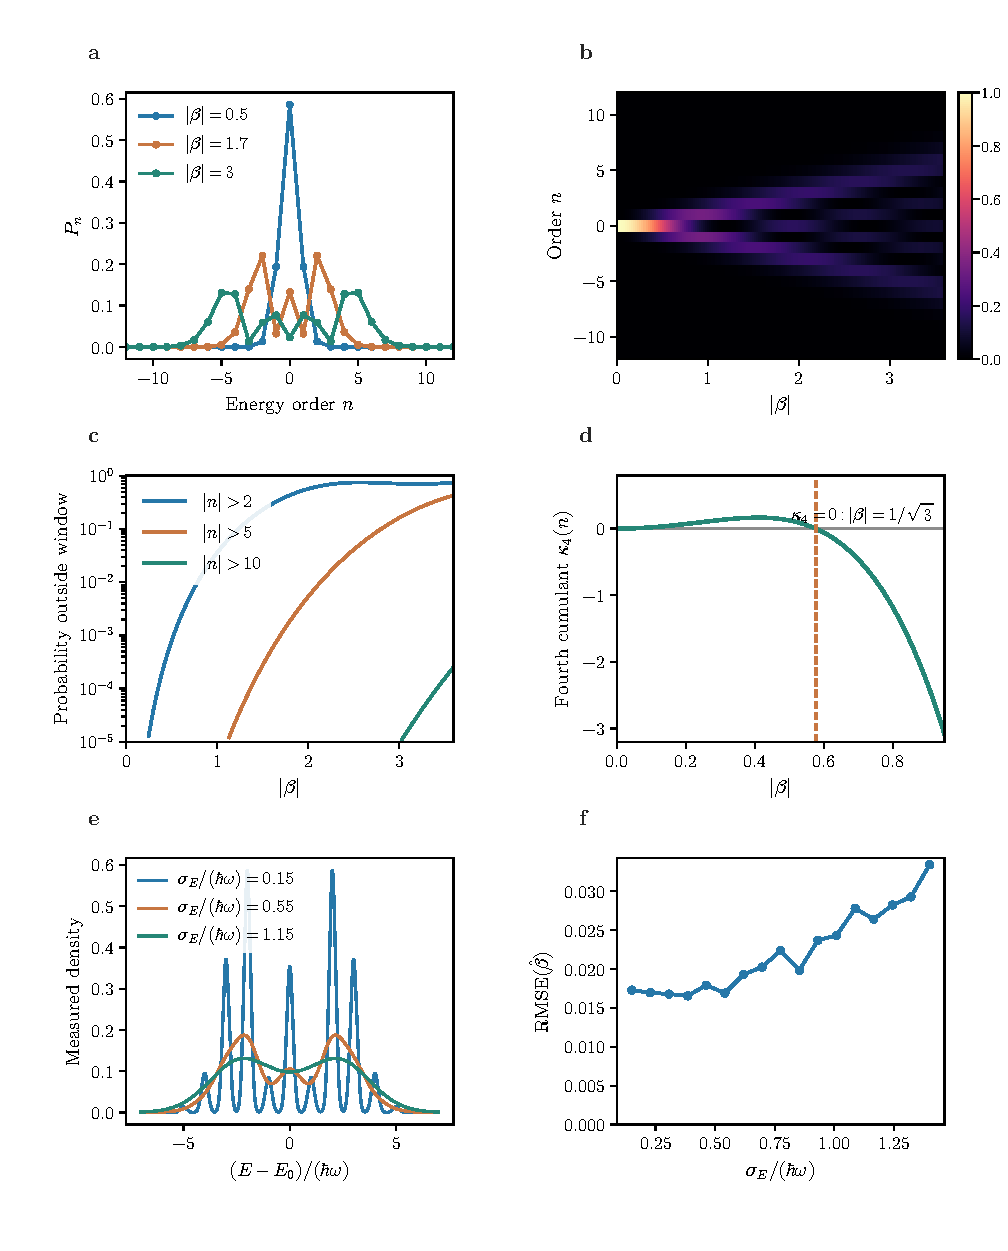
\includegraphics[width=0.97\linewidth,height=0.70\textheight,keepaspectratio]{sideband_moments_and_resolution.pdf}
\caption{\textbf{贝塞尔谱矩如何进入实际测量。} (a) 三种耦合强度的完整边带概率；(b) 随耦合演化的阶数分布及贝塞尔零点；(c) 有限能量收集窗口 $|n|\leq2,5,10$ 遗漏的概率随耦合增强而增长；(d) 由贝塞尔特征函数计算的非高斯第四累积量及其零点；(e) 同一真实概率分布在不同探测器分辨率下的卷积谱；(f) 有限电子计数下，用已知探测器方差反演耦合强度的均方根误差。所有面板由同一贝塞尔模型生成，探测器仅引入独立高斯展宽。}
\label{fig:pinem-sideband-moments-resolution}
\end{figure}

图中 (a)--(d) 采用 $n=-24,\ldots,24$ 的求和截断，其中 (a) 固定 $b=0.5,1.7,3.0$，(b)--(d) 扫描 $b\in[0,3.6]$ 共 160 点；(c) 按 $\sum_{|n|>n_{\max}}P_n$ 计算遗漏概率，仅展示高于 $10^{-5}$ 的部分；(d) 仅显示 $b\in[0,0.95]$，标出 $b=1/\sqrt3$ 处第四累积量变号。所有离散概率都按有限和重新归一，并通过扩大截断检查收敛。(e) 固定 $b=1.7$，用单位面积响应 $G_s(Y-n)=\exp[-(Y-n)^2/(2s^2)]/(\sqrt{2\pi}s)$ 在 $Y\in[-7,7]$ 的 1600 点网格卷积，比较 $s=0.15,0.55,1.15$；所画纵轴始终是归一化概率密度。(f) 同样固定 $b=1.7$，扫描 $s\in[0.15,1.40]$ 共 17 点，对每一取值独立模拟 140 批、每批 1800 次电子能量记录，随机数种子为 2409；由 $\widehat b=\sqrt{\max(\frac1N\sum_jY_j^2-s^2,0)/2}$ 反演后，再计算 140 批的均方根误差。这里假定 $E_0$ 和探测器响应宽度已经标定，未加入空间束斑平均、背景和计数损失。


边带概率只要求电子在固定的正能支上满足窄谱、弱反冲近似；电子自旋量随动量变化所产生的投影和归一化修正由后面的 Dirac 动力学确定。


在电子一侧，我们已经从一阶包络的受控条件推到轨迹相位、贝塞尔边带和可测谱矩。接下来必须进一步区别两件事：电子真正受到的局域场强如何随横向位置变化，以及不同位置的概率在实际电子束与仪器中怎样平均。只有完成这一步，理论才能回答一个实验中最直接的问题：为什么相同照明功率下，改变结构、撞击位置或探测器分辨率会得到不同的 PINEM 图像。
